%% Font size %%
\documentclass[11pt]{article}

%% Load the custom package
\usepackage{Mathdoc}

%% Numéro de séquence %% Titre de la séquence %%
\renewcommand{\centerhead}{Chapitre 01 : Nombres relatifs - Bataille navale}

%% Spacing commands %%
\renewcommand{\baselinestretch}{1} \setlength{\parindent}{0pt}

%% Quadrillage relatif -10 à +10, avec label centré au-dessus, axes fléchés et graduation +1/-1 %%
\newcommand{\grillerelatifs}[1]{%
\begin{center}
\textbf{\large #1}\\[0.4em]
\resizebox{\linewidth}{!}{%
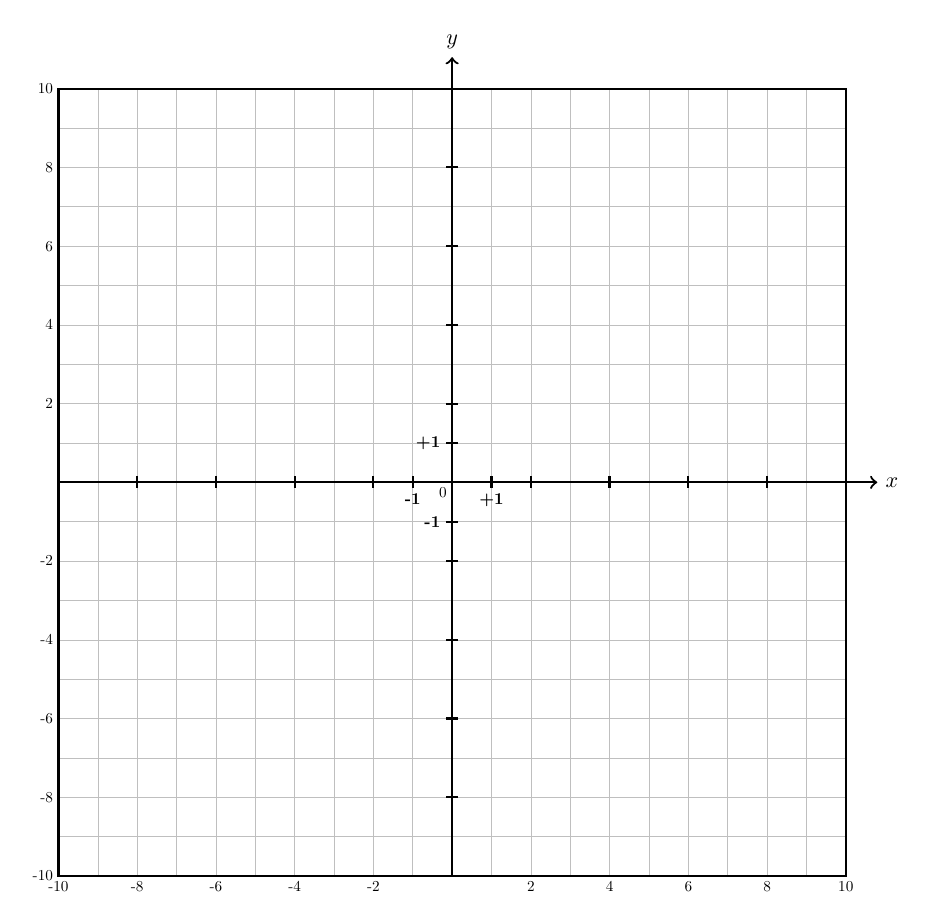
\begin{tikzpicture}[x=0.5cm,y=0.5cm]
\draw[step=1,gray!50,very thin] (-10,-10) grid (10,10);
\draw[thick] (-10,-10) rectangle (10,10);
\draw[->,thick] (-10,0) -- (10.8,0) node[right,scale=0.8] {$x$};
\draw[->,thick] (0,-10) -- (0,10.8) node[above,scale=0.8] {$y$};
\foreach \v in {-10,-8,...,-2,2,4,...,10}{
\node[below,scale=0.55] at (\v,-10) {\v};
\node[left,scale=0.55] at (-10,\v) {\v};
\draw[thick] (\v,0.15) -- (\v,-0.15);
\draw[thick] (0.15,\v) -- (-0.15,\v);
}
\node[below left,scale=0.55] at (0,0) {0};
\draw[thick] (1,0.15) -- (1,-0.15);
\node[below,scale=0.6] at (1,-0.15) {\textbf{+1}};
\draw[thick] (-1,0.15) -- (-1,-0.15);
\node[below,scale=0.6] at (-1,-0.15) {\textbf{-1}};
\draw[thick] (0.15,1) -- (-0.15,1);
\node[left,scale=0.6] at (-0.15,1) {\textbf{+1}};
\draw[thick] (0.15,-1) -- (-0.15,-1);
\node[left,scale=0.6] at (-0.15,-1) {\textbf{-1}};
\end{tikzpicture}}
\end{center}}

%% Petit dessin de bateau : #1 = nb de cases, #2 = nom, #3 = taille d'une case (cm) %%
\newcommand{\bateau}[3]{%
\pgfmathtruncatemacro{\last}{#1-1}%
\begin{tikzpicture}[x=#3cm,y=#3cm,baseline=(current bounding box.south)]
\foreach \i in {0,...,\last}{
\draw[fill=gray!20,thick] (\i,0) rectangle ++(1,1);
}
\draw[fill=gray!55,thick] (\last,0) -- (#1,0.5) -- (\last,1) -- cycle;
\node[below,scale=0.65] at (#1/2,-0.35) {\textbf{#2}};
\node[below,scale=0.55] at (#1/2,-0.95) {(#1 cases) $\square$};
\end{tikzpicture}}

\begin{document}

\textbf{\LARGE Bataille navale des relatifs}\\[0.3em]

\begin{rappel}
\begin{minipage}[c]{0.56\linewidth}
Un \textbf{repère} est formé de deux axes gradués et perpendiculaires qui
se coupent à l'origine $O$.
\begin{itemize}[itemsep=1pt,topsep=2pt]
\item L'axe horizontal est l'\textbf{axe des abscisses}.
\item L'axe vertical est l'\textbf{axe des ordonnées}.
\end{itemize}
Un point $M$ du plan est repéré par un couple de nombres relatifs
$(x\,;\,y)$ appelé ses \textbf{coordonnées} : $x$ est
l'\textbf{abscisse} de $M$ (on la lit sur l'axe horizontal), $y$ est
son \textbf{ordonnée} (on la lit sur l'axe vertical).
\end{minipage}\hfill
\begin{minipage}[c]{0.4\linewidth}
\centering
\begin{tikzpicture}[x=0.6cm,y=0.6cm]
\draw[->,thick] (-1.5,0) -- (5,0) node[right,scale=0.7] {$x$};
\draw[->,thick] (0,-1.5) -- (0,4.5) node[above,scale=0.7] {$y$};
\foreach \i in {-1,1,2,3,4}{\draw (\i,0.1) -- (\i,-0.1);}
\foreach \j in {-1,1,2,3,4}{\draw (0.1,\j) -- (-0.1,\j);}
\node[below left,scale=0.6] at (0,0) {0};
\node[below,scale=0.6] at (1,-0.1) {1};
\node[left,scale=0.6] at (-0.1,1) {1};
\draw[dashed] (3,0) -- (3,2) -- (0,2);
\fill (3,2) circle (2pt);
\node[above right,scale=0.7] at (3,2) {$M(3\,;\,2)$};
\node[below,scale=0.6] at (3,0) {3};
\node[left,scale=0.6] at (0,2) {2};
\end{tikzpicture}
\end{minipage}
\end{rappel}

\smallskip

Toute la classe affronte le professeur ! Chacun·e place secrètement ses
bateaux sur son quadrillage \textit{Mes bateaux}. À chaque tour :
\begin{itemize}[itemsep=0pt,topsep=2pt]
\item un·e élève donne une coordonnée pour attaquer la grille du
professeur : on la note sur le quadrillage \textit{J'attaque le
professeur} ;
\item le professeur annonce ensuite une seule coordonnée qui attaque
\textbf{toute la classe en même temps} : vérifie si elle touche un de tes
bateaux sur \textit{Mes bateaux}.
\end{itemize}
Le professeur répond \textbf{à l'eau}, \textbf{touché} ou \textbf{coulé}
(quand toutes les cases d'un bateau sont touchées). Une coordonnée
s'écrit $(x\,;\,y)$, par exemple $(-3\,;\,+5)$.

\smallskip

\noindent
\begin{minipage}[t]{0.44\linewidth}
\grillerelatifs{J'attaque le professeur}
\end{minipage}\hfill
\begin{minipage}[t]{0.44\linewidth}
\grillerelatifs{Mes bateaux}
\end{minipage}

\smallskip

\textbf{\large Comment placer ses bateaux ?}
\begin{itemize}[itemsep=3pt,topsep=6pt]
\item Chaque bateau occupe des cases alignées, à l'horizontale ou à la
verticale (jamais en diagonale).
\item Deux bateaux ne peuvent jamais se toucher, même par un coin.
\item Place les 5 bateaux ci-dessous sur ton quadrillage \textit{Mes
bateaux}, puis coche-les au fur et à mesure.
\end{itemize}

\smallskip

\begin{center}
\bateau{5}{Porte-avions}{0.5}\qquad
\bateau{4}{Croiseur}{0.5}\qquad
\bateau{3}{Contre-torpilleur}{0.5}\qquad
\bateau{3}{Sous-marin}{0.5}\qquad
\bateau{2}{Torpilleur}{0.5}
\end{center}

\end{document}
